\begin{figure*}
\ifthenelse{\boolean{plosone}}{
  \begin{adjustwidth}{-2.25in}{0in}
}{}
 % Comment out/remove adjustwidth environment i

\begin{tabular}{p{0.5\textwidth}p{0.5\textwidth}}
{\sf \large A} & {\sf \large B}
\\
\vspace{0pt}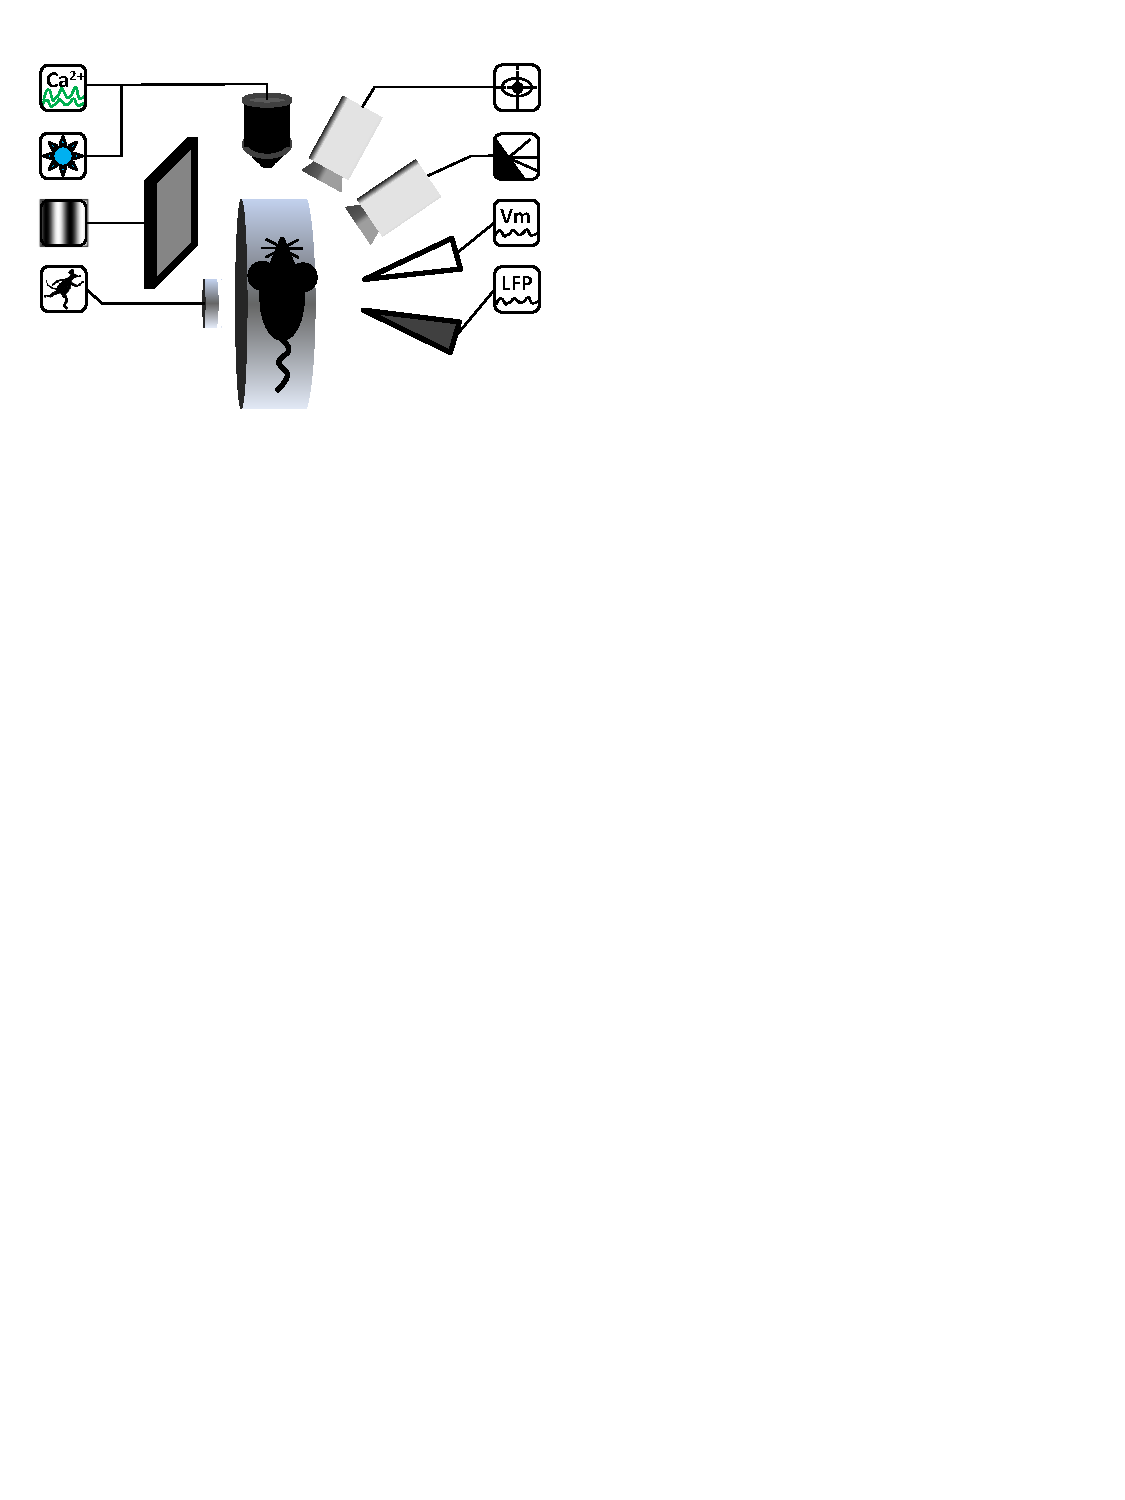
\includegraphics{./figures/experiment.pdf} &
\vspace{0pt}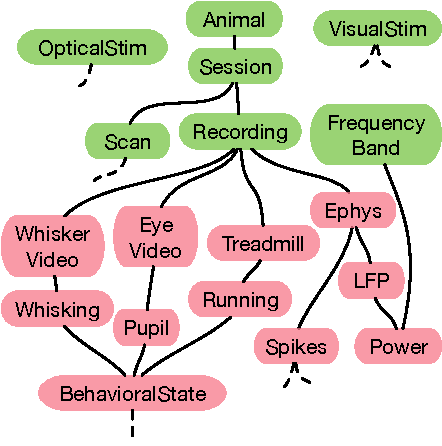
\includegraphics{./figures/schema.pdf}
\\
\end{tabular}

{\sf \large C}
\vspace{6pt}

\inputminted[frame=single,linenos=true]{python}{Session.py}

\vspace{6pt}
{\sf \large D}
\vspace{6pt}

\csvreader[
table head = \hline\bf animal & \bf session & \bf user & \bf session\_date & \bf session\_folder & \bf notes & \bf timestamp\\\hline,
before table=\rowcolors{1}{white}{Beige},
table foot = \hline,
head to column names,
tabular=|cc|lllll|
]{session.csv}{}%
{\tt\animal & \tt\session & \tt\user & \tt\date & \tt\folder & \tt\notes & \tt\ts}
\caption{
{\bf An example experiment and its DataJoint schema.}
{\sf A.}  
A neuroscience experiment with multiple stimulation and acquisition modalities (counterclockwise from top left corner): fluorescence imaging of calcium signals (Ca$^{2+}$), light stimulation of optogenetic probes, visual stimulus, treadmill motion recording, local-field potential recording (LFP), whole-cell patch membrane potential recording (V\textsubscript{m}), video of whisker movements, video of eye movements.
{\sf B.}  The entity relationship diagram (ERD) of a DataJoint schema comprising base relations storing externally entered data (green) and automatically populated data (red).
{\sf C.}  
The Python class for the base relation \mintinline{python}{Session} specifying the relation's heading. 
A dependency on \mintinline{python}{Animal} is indicated with the arrow {\tt-\textgreater}.  
An additional primary key attribute, {\tt session}, enables multiple sessions per animal. 
Dependent attributes are separated from primary key attributes by {\tt---}.   
Each attribute has a name, an optional default value, a datatype, and an optional comment.
{\sf D.}  
Example contents of \mintinline{python}{Session}.
The vertical divider separates the primary key attributes `{\tt animal}' and `{\tt session}` from the dependent attributes.
} 
\label{schema}
\ifthenelse{\boolean{plosone}}{\end{adjustwidth}}{}
\end{figure*}
